\documentclass[10pt,pdf,aspectratio=169]{beamer}
\usetheme{CambridgeUS}

\usepackage{graphicx}

\usepackage{caption}
\captionsetup[figure]{labelformat=empty}% redefines the caption setup of the figures environment in the beamer class.

%\setbeamertemplate{caption}{\raggedright\insertcaption\par}

% \usepackage{dsfont}
\usepackage{cancel}
\usepackage[export]{adjustbox}
\usepackage{amsthm}
\usepackage{amsmath}
%\usepackage{stmaryrd}
\usepackage{ulem}
% \usepackage[backend=biber,style=numeric-comp,sorting=none]{biblatex}
\usepackage{stmaryrd}
\usepackage[english]{babel}
\usepackage{fontspec}
\usepackage[]{graphics}
\usepackage{mathtools}
\usepackage{cite}
\usepackage{hyperref}

\setmainfont{cmun}[
  Extension=.otf,
  UprightFont=*rm,
  ItalicFont=*ti,
  BoldFont=*bx,
  BoldItalicFont=*bi,
]
\setsansfont{cmun}[
  Extension=.otf,
  UprightFont=*ss,
  ItalicFont=*si,
  BoldFont=*sx,
  BoldItalicFont=*so,
]
\setmonofont{cmun}[
  Extension=.otf,
  UprightFont=*btl,% light version
  ItalicFont=*bto,%  light version
  BoldFont=*tb,
  BoldItalicFont=*tx,
]

\usepackage{tikz}
\usepackage[beamer]{hf-tikz}
\usepackage{pgfplots}
\usepackage{ragged2e}
\usepackage{bbm}

\usetikzlibrary{arrows,automata,shapes,calc,patterns,arrows.meta}
\usetikzlibrary{fadings}

\usepackage{subfig}
% \pgfplotsset{
%   axis line style={thick, black!50},
% }
\tikzset{
  every picture/.style={line width=1pt},
  >=latex
}

\makeatother
\title[Перетворення відеозапису з дошки у слайд-шоу]{
  \huge{Перетворення відеозапису з дошки у слайд-шоу}
}

\author[Доповідач: Максим Шило,  Науковий керівник: Водолазський Є. В.]{
Доповідач: Максим Шило\inst{1} \and
Науковий керівник: Водолазський Є. В.\inst{1}}

\institute{
  \inst{1} Національний технічний університет України
  ``Київський політехнічний інститут імені Ігоря Сікорського''}

\date[]{16 червня 2022}

\setbeamertemplate{theorems}[numbered]

\DeclareMathOperator{\argmax}{argmax}
\DeclareMathOperator{\argmin}{argmin}
\DeclareMathOperator{\rank}{rank}

% \bibliographystyle{plain}
% \addbibresource{proofs}
% \bibliography{proofs}

\begin{document}

\begin{frame}
  \titlepage
\end{frame}

\begin{frame}
    \frametitle{Мотивація}
    \begin{figure}
        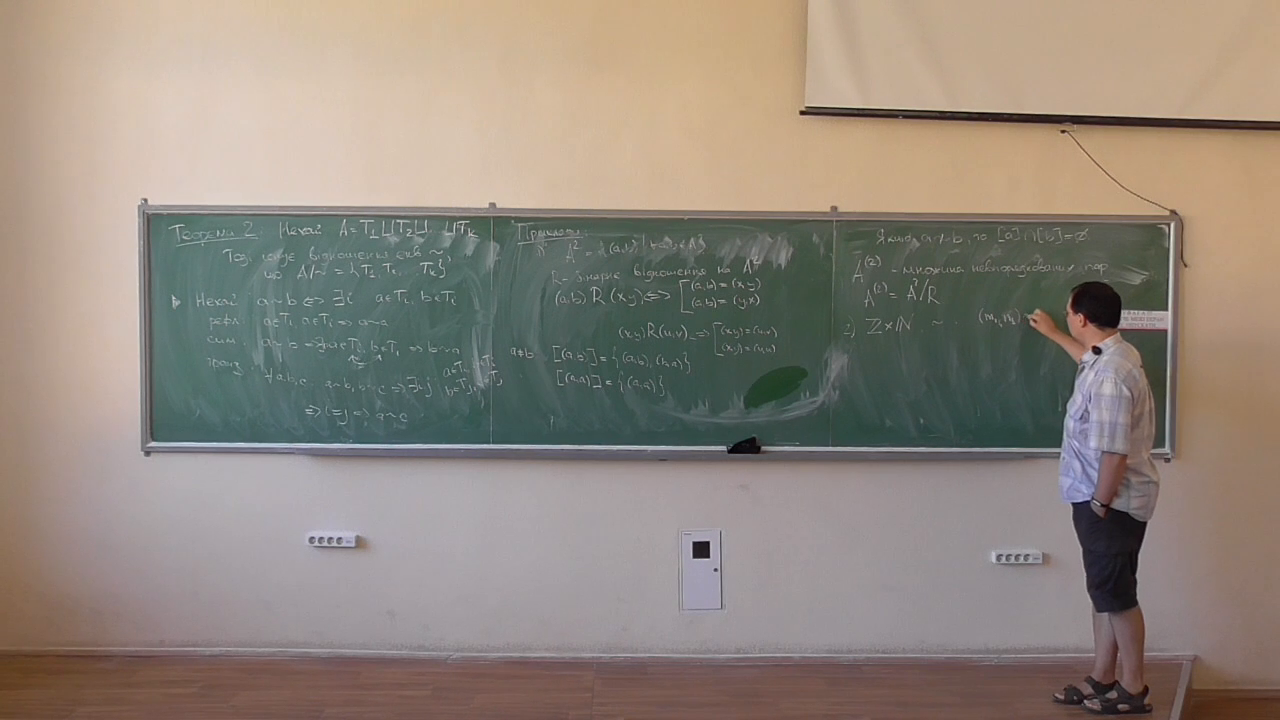
\includegraphics[width=0.4\textwidth]{images/before.png}
    \end{figure}
    \begin{figure}
        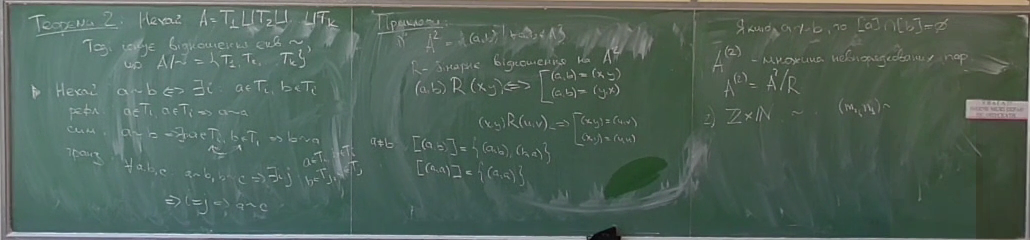
\includegraphics[width=0.7\textwidth]{images/after.png}
        \caption{Джерело ~---~\url{https://youtu.be/a7TUp4p-pIk}
        }
    \end{figure}

\end{frame}

\begin{frame}
    \frametitle{Мотивація}
    \begin{figure}
        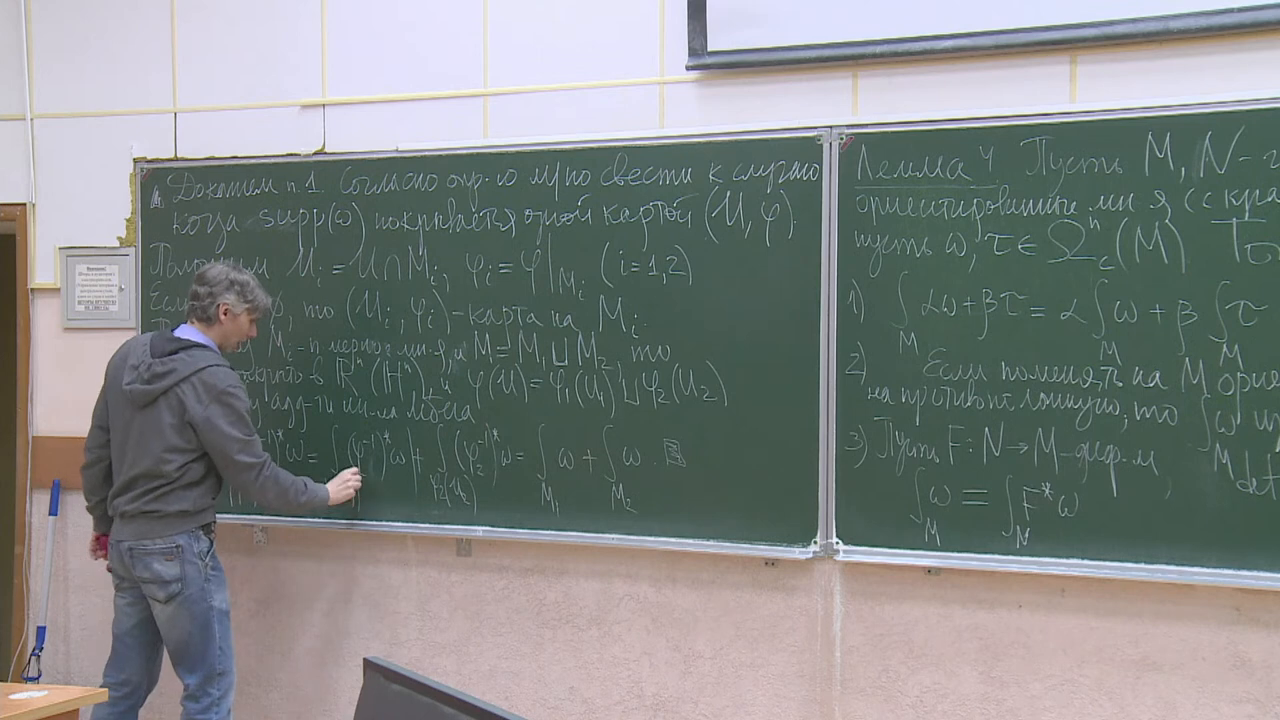
\includegraphics[width=0.3\textwidth]{images/kratnye_intergraly_left.png}
        \quad
        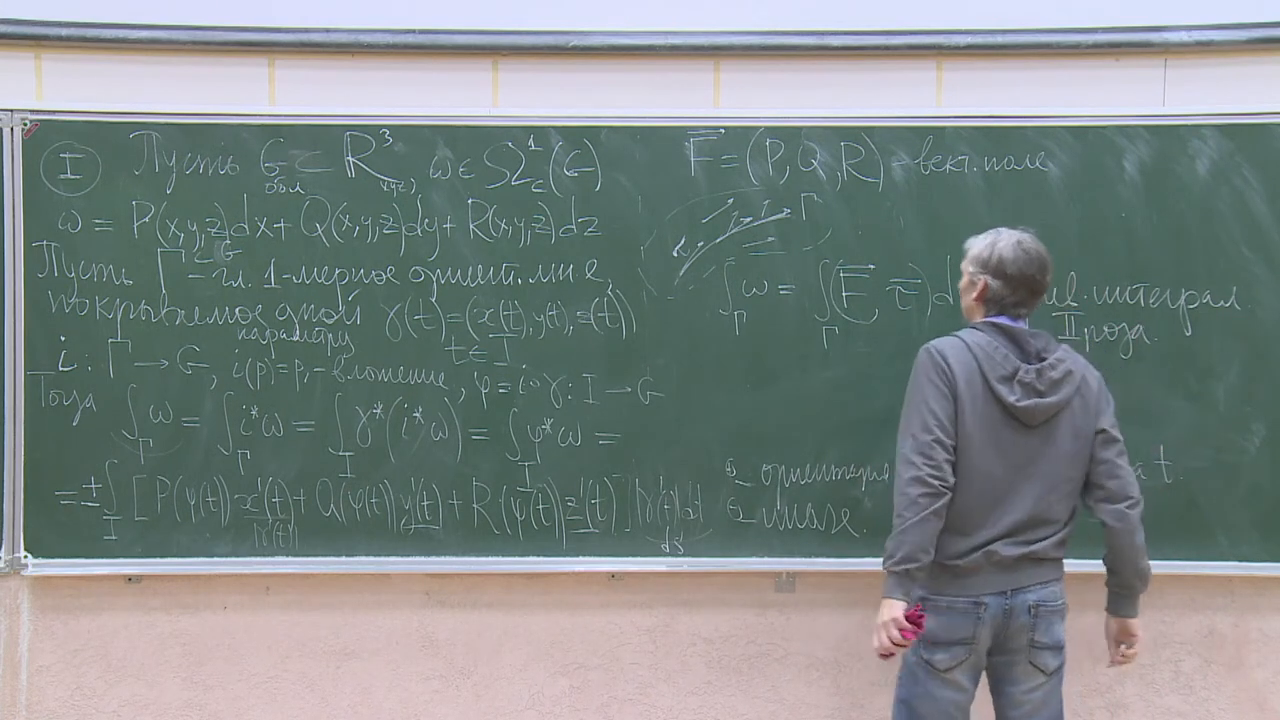
\includegraphics[width=0.3\textwidth]{images/kratnye_intergraly_center.png}
        \quad
        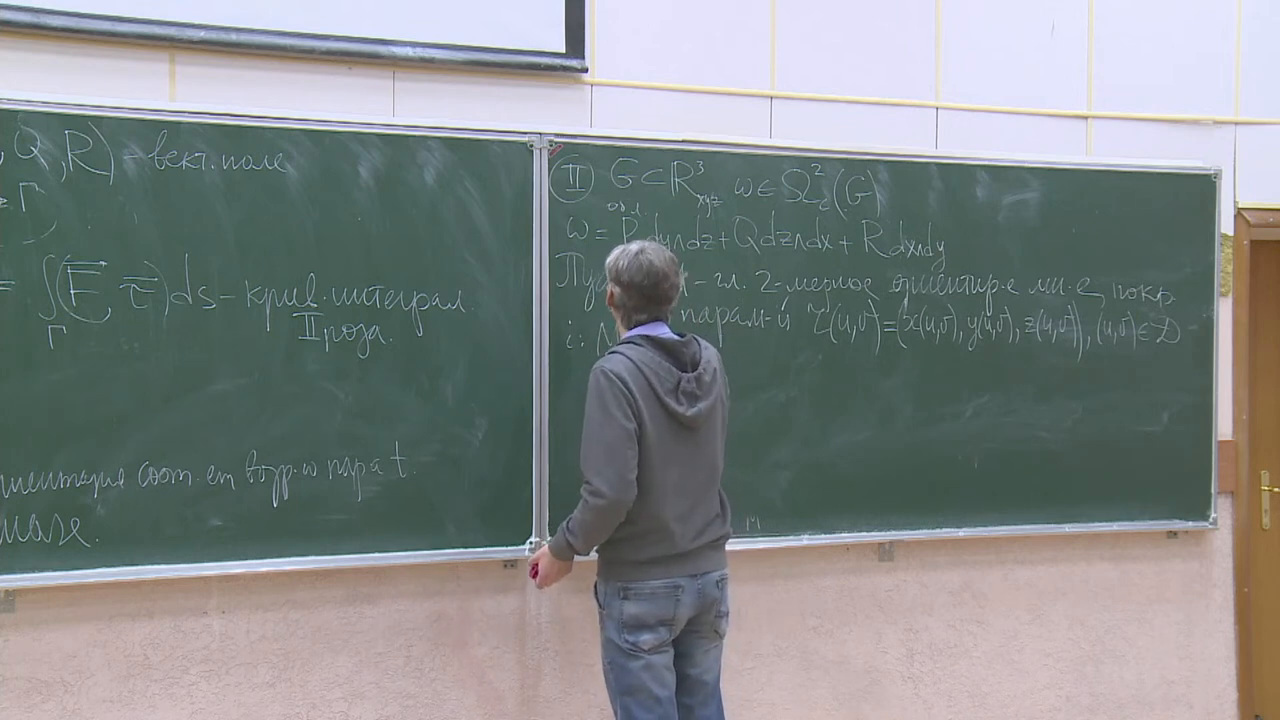
\includegraphics[width=0.3\textwidth]{images/kratnye_intergraly_right.png}
    \end{figure}
    \begin{figure}
        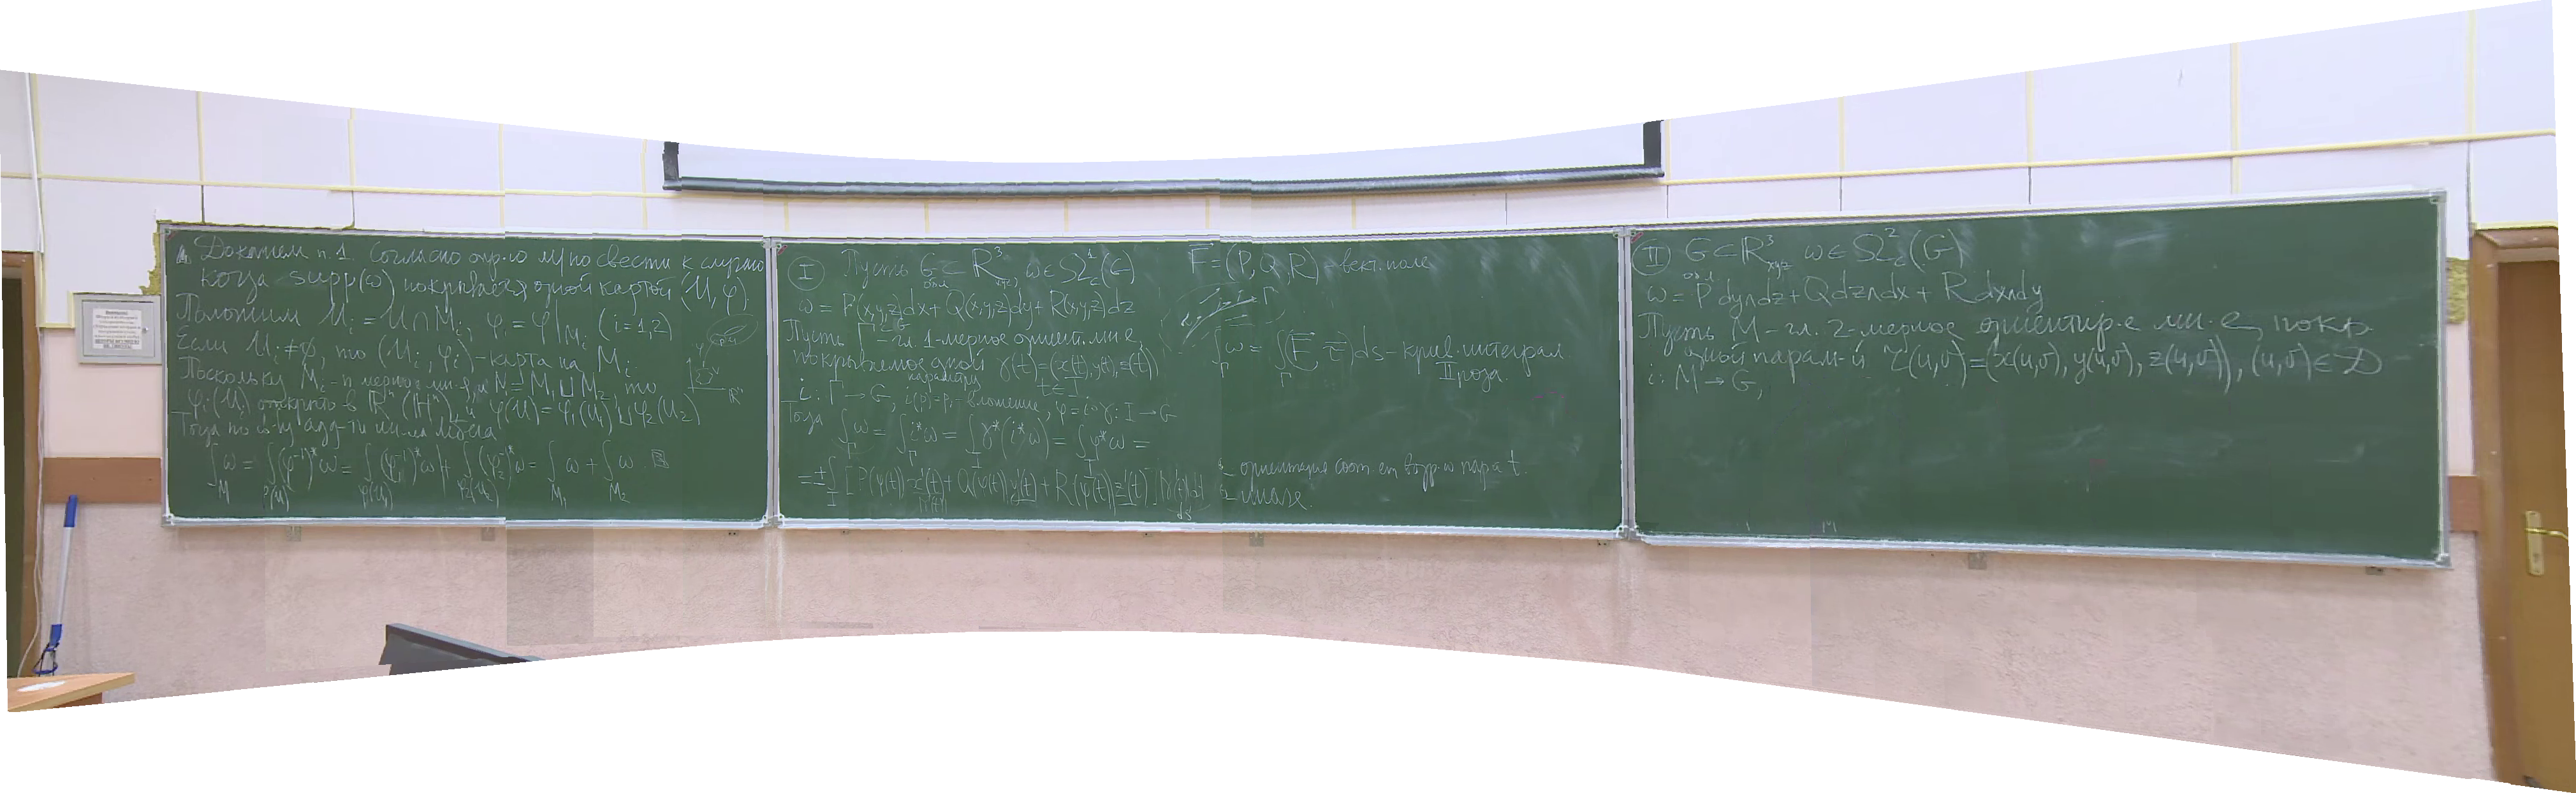
\includegraphics[width=0.8\textwidth]{images/kratnye_integraly_panorama.png}
    \end{figure}
\end{frame}

\begin{frame}
    \frametitle{Вступ}
    \textbf{Об'єкт дослідження}~---~відеозаписи лекцій. \\
    \textbf{Предмет дослідження}~---~автоматична обробка відеозаписів. \\ 
    \textbf{Метою роботи} є розробка інформаційної технології, що перетворює 
    відеозапис лекції у панорамні знімки без викладача. \\

    Дана інформаційна технологія повинна мати ряд властивостей:
    \begin{itemize}
        \item здатність працювати на звичайному смартфоні у режимі реального часу;
        \item можливість працювати з дошками різного кольору;
        \item можливість працювати з рухливою камерою;
        \item мінімальна кількість дефектів на слайдах,
            таких як наявність фрагментів викладача
            або видимі шви у місцях склейки кадрів.
    \end{itemize}
\end{frame}

\setbeamertemplate{section in toc}{\inserttocsectionnumber~\inserttocsection}
\pagenumbering{}
\begin{frame}
  \frametitle{Зміст}
    \tableofcontents
\end{frame}

\section{Процедура створення панорамних слайдів}
\begin{frame}
    \frametitle{Процедура створення панорамних слайдів}
    \usetikzlibrary{arrows,positioning,shapes}
    \begin{figure}[H]
        \begin{center}
            \begin{tikzpicture}[node distance=4mm, >=latex',
                    block/.style = {draw, rectangle, minimum height=10mm, minimum width=28mm,align=center},
                    rblock/.style = {draw, rectangle, rounded corners=0.5em},
                    tblock/.style = {draw, trapezium, minimum height=10mm,
                            trapezium left angle=75, trapezium right angle=105, align=center},
                ]
                \node [rblock]                           (video)        {Відео};
                \node [block, below=of video]            (mov_objects)  {Побудова маски\\
                    рухомих об'єктів або людини};
                \node [block, right=of mov_objects]      (pan)          {Побудова панорамами};
                \node [block, right=of pan]              (denoise)      {Зниження рівня\\ шуму};
                \node [rblock,above=of denoise]          (slides)       {Слайди};

                \path[draw,->] (video)         edge    (mov_objects)
                (mov_objects)   edge    (pan)
                (pan)           edge    (denoise)
                (denoise)       edge    (slides)
                ;
            \end{tikzpicture}
        \end{center}
    \end{figure}
\end{frame}

\section{Стабілізація відео}
\begin{frame}
  \frametitle{Стабілізація відео}

  Оскільки дошка~---~це плоска поверхня, ми можемо знайти матрицю гомографії між двома кадрами.
  Для цього використовуємо алгоритм SIFT та RANSAC.
  \begin{figure}[H]
    \centering
    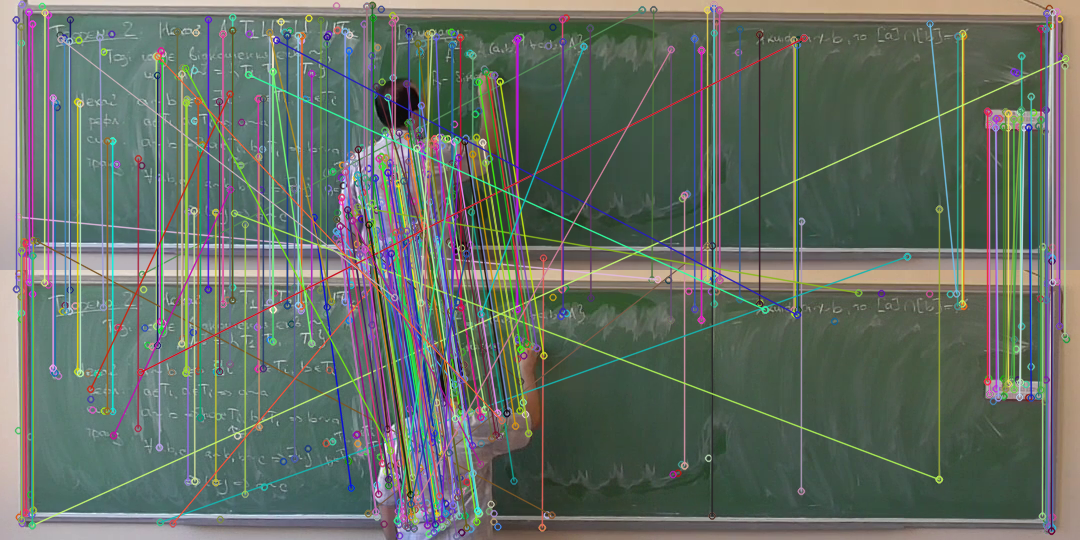
\includegraphics[width=0.55\textwidth]{images/matches_img}
    \caption{Кадри $F^i$ (верхній) та $F^{i+s}$ (нижній) із ключовими точками та лініями, \\
      які поєднують відповідні точки з відео
    }
  \end{figure}

\end{frame}

\section{Методи локалізації людини та рухомих об'єктів}
\begin{frame}
  \frametitle{Алгоритм Бойкова Колмогорова}

  Сформулюємо задачу максимального потоку
  \begin{equation*}
    \sum_{t \in N_s} f_{st} \rightarrow \max_{f: \tau \rightarrow R }
  \end{equation*}
  з обмеженнями
  \begin{equation*}
    \begin{gathered}
      \begin{cases}
        f_{tt^{'}} \leq  c_{tt^{'}},                                   & \forall tt^{'}  \in \tau ,         \\
        \sum_{p \in P_t} f_{pt} - \sum_{t^{'} \in N_t} f_{tt^{'}} = 0, & \forall t \in T \setminus \{s,e\}, \\
        \sum f_{tt^{'}} \geq 0,                                        & \forall tt^{'}  \in \tau.
      \end{cases}
    \end{gathered}
  \end{equation*}
  Це означає, що
  \begin{enumerate}
    \item потік має не перевищувати пропускну здатність для всіх ребер;
    \item сума потоків, що входять у вузол не повинна змінитись на виході;
    \item потік завжди додатній.
  \end{enumerate}
\end{frame}

\section{Методи локалізації людини та рухомих об'єктів}
\begin{frame}
  \frametitle{Процес створення маски рухомих об'єктів алгоритмом Б-К}
  
  \begin{figure}[H]
	\centering
	\subfloat[Попередній кадр $F^i$]{
		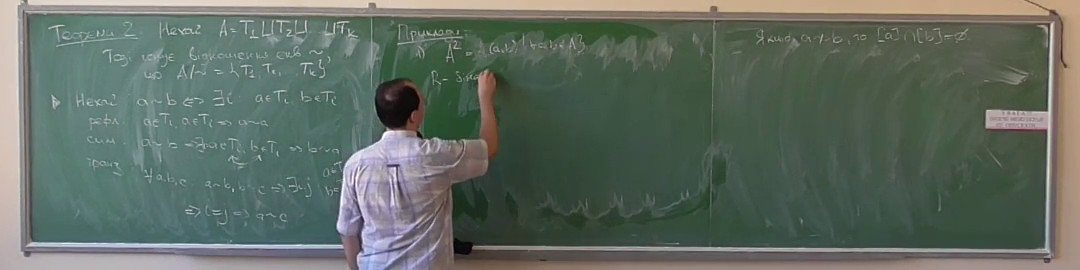
\includegraphics[width=0.45\textwidth]{images/prev_frame}
	}\\
	\subfloat[Поточний кадр $F^{i+s}$]{
		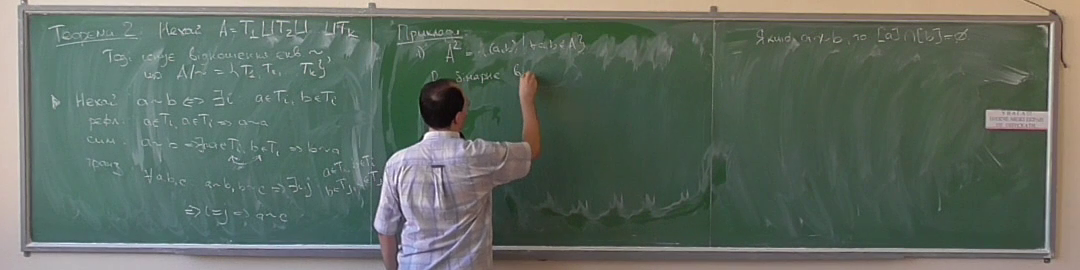
\includegraphics[width=0.45\textwidth]{images/next_frame}
	}\\
	\subfloat[Інвертована різниця $F^i$ і $F^{i+s}$]{
		
\includegraphics[width=0.45\textwidth]{images/inv_diff}
	}\\
	\subfloat[Маска рухомих об'єктів на кадрі $F^{i+s}$]{
		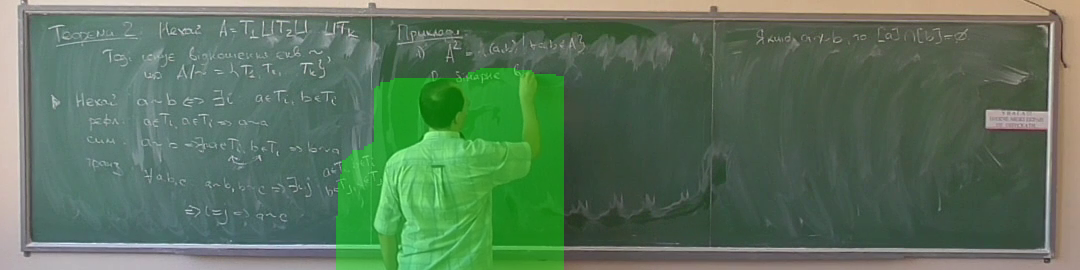
\includegraphics[width=0.45\textwidth]{images/next_with_mask}
	}
\end{figure}
\end{frame}

\begin{frame}
  \frametitle{Згорткові нейронні мережі для локалізації людини}

  \begin{figure}[H]
    \centering
    \subfloat[Алгоритм Б-К]{
      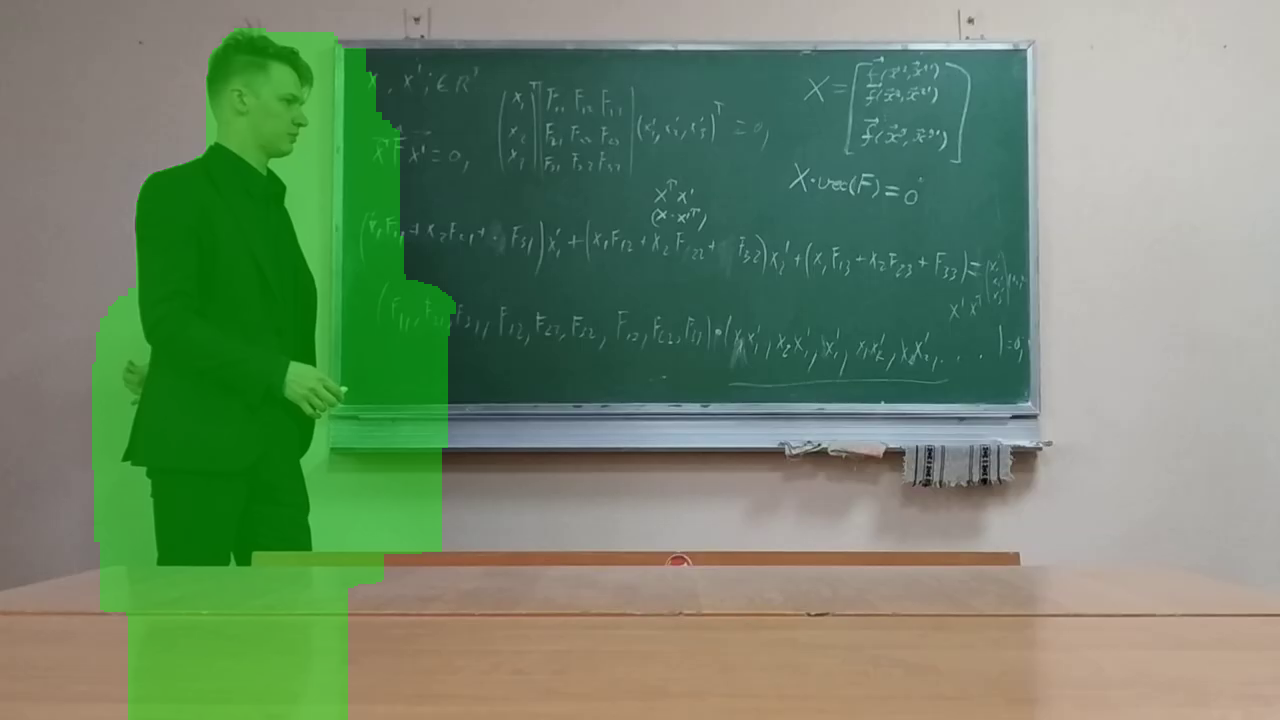
\includegraphics[width=0.3\textwidth]{images/krygin_geometry_bk_17350}
    }
    \subfloat[yolov5n]{
      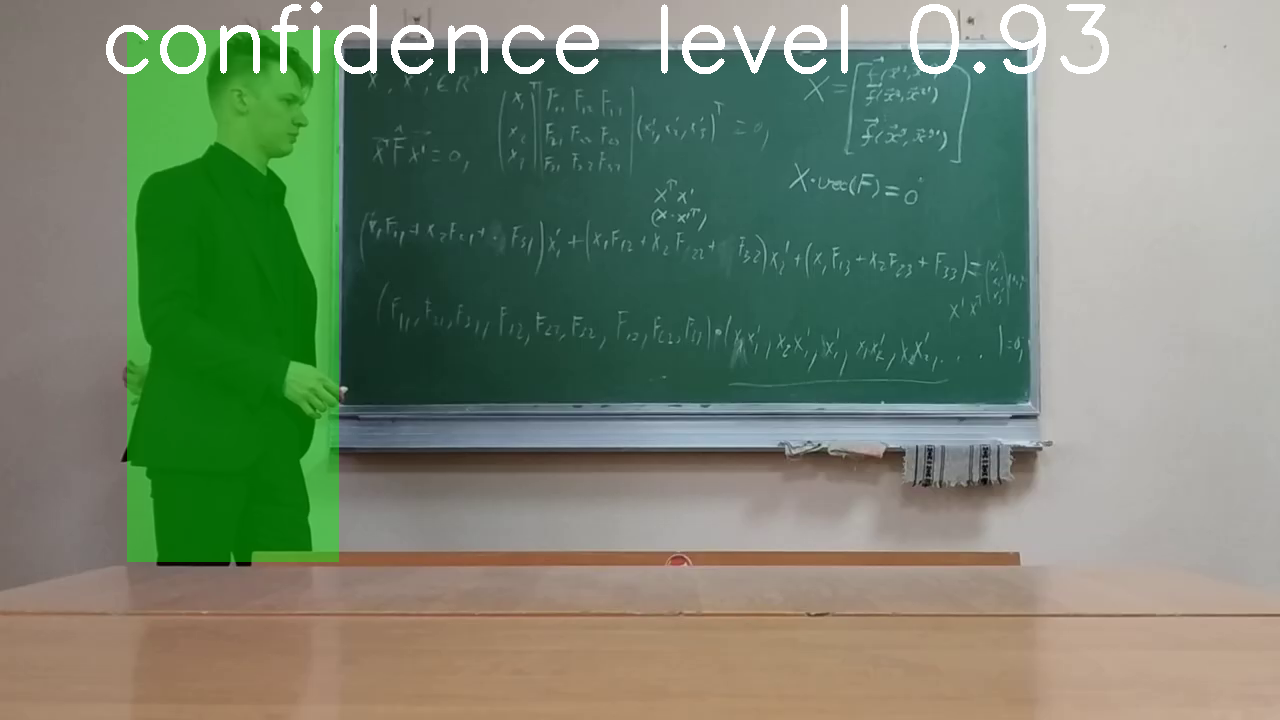
\includegraphics[width=0.3\textwidth]{images/krygin_geometry_yolov5n_17350}
    }\\
    \subfloat[ssdlite320-mobilenet-v3]{
      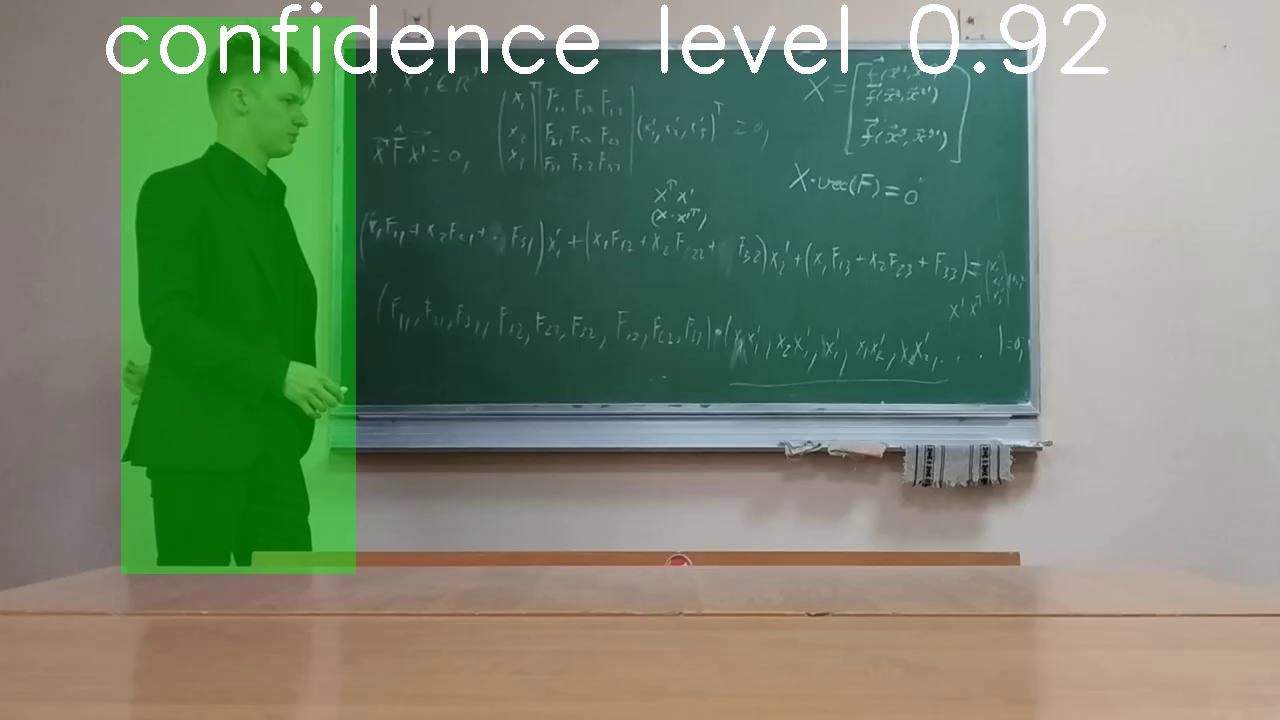
\includegraphics[width=0.3\textwidth]{images/krygin_geometry_ssdlite320_mobilenet_v3_17350}
    }
    \subfloat[fasterrcnn-mobilenet-v3]{
      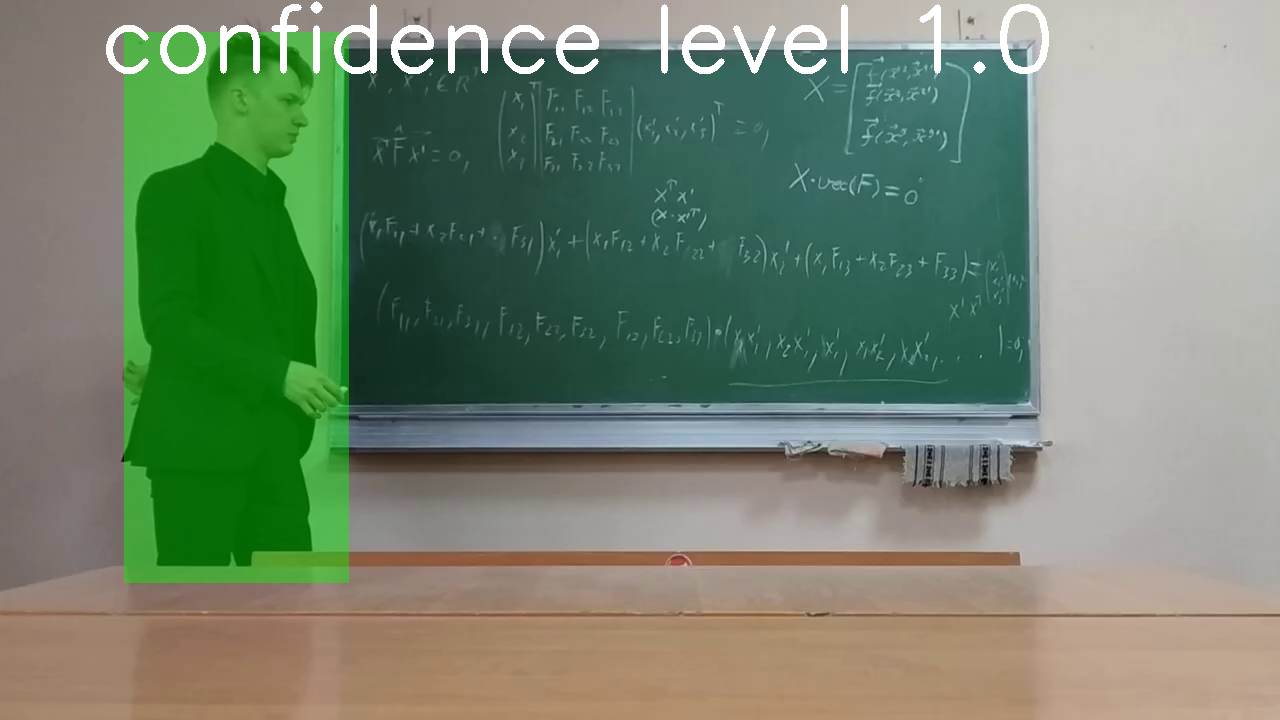
\includegraphics[width=0.3\textwidth]{images/krygin_geometry_fasterrcnn_mobilenet_v3_17350}
    }
    % \caption{Приклад роботи методів локалізації людини та рухомих об'єктів
    % }
  \end{figure}
\end{frame}

\section{Створення панорами}
\begin{frame}
  \frametitle{Алгоритм створення панорами}
  \textbf{Вхід:} два кадри \(F^{i}\) та \(F^{i + s}\), поточна панорама \(W^{i}\) (\(W^{1} = F^{1}\)). \\
  \textbf{Вихід:} панорама \(W^{i + s}\). \\
  \textbf{Етап отримання відповідних точок.} \\
  \textbf{1.}
  Знаходимо набір \(M^{i}\) пар відповідних пікселів між кадрами
  \(F^{i}\) і \(F^{i + s}\) і будуємо множину
  \(M^{'i} = \left\{ \left( p^{i},p^{i + s} \right) \in M^{i}:B_{p^{i}}^{i} = B_{p^{i + s}}^{i} = 0 \right\}\)
  тих пар відповідних пікселів, координати яких не належать області
  рухомих об'єктів.\\

  \textbf{2.}
  Якщо \(\left| {M'}^{i} \right| < 0.5 \cdot \left| M^{i} \right|\) або
  \(\left| {M'}^{i} \right| < 4\), завершуємо алгоритм з результатом
  \(W^{i + s} = W^{i}\).\\

  \textbf{3.}
  Знаходимо набір \(M_{W}^{i}\) пар відповідних пікселів між панорамою
  \(W^{i}\) і кадром \(F^{i + s}\) і будуємо множину
  \(M_{W}^{'i} = \left\{ \left( p_{W}^{i},p^{i + s} \right) \in M_{W}^{i}:\exists p^{i} \in P:\left( p^{i},p^{i + s} \right) \in M^{'i} \right\}\). \\

  \textbf{Етап обчислення матриці гомографії.}\\
  \textbf{4.}
  На базі множини \(M_{W}^{'i}\) пар відповідних точок знаходимо матрицю
  \(H_{W}^{i}\) гомографії, що співставляє пікселі кадру \(F^{i + s}\)
  та панорами \(W^{i}\). \\

  \textbf{Етап обчислення розміру нової панорами.} \\
  \textbf{5.}
  Рахуємо координати крайніх точок кадру \(F^{i + s}\) після застосування до них матриці
  \(H_{W}^{i}\).
  $l_{1}^{i} = H_{W}^{i} \cdot (0,0,1)^{T}, l_{2}^{i} = H_{W}^{i} \cdot (w - 1,0,1)^{T},  l_{3}^{i} = H_{W}^{i} \cdot (0,h - 1,1)^{T},l_{4}^{i} = H_{W}^{i} \cdot (h - 1,h - 1,1)^{T}$
 
\end{frame}

\begin{frame}
    \frametitle{Алгоритм створення панорами}
    \textbf{6.}
    Для визначення множини \(P_{W}^{i}\) нової панорами \(W^{i + s}\)
    рахуємо величини
    $
        x_{\min}^{i} = \min_{j = \overline{1,4}}\frac{( l_{j}^{i} )_{x}}{( l_{j}^{i} )_{z}},
        x_{\max}^{i} = \max_{j = \overline{1,4}}\frac{( l_{j}^{i} )_{x}}{( l_{j}^{i} )_{z}},
        y_{\min}^{i} = \min_{j = \overline{1,4}}\frac{( l_{j}^{i} )_{y}}{( l_{j}^{i} )_{z}},
        y_{\max}^{i} = \max_{j = \overline{1,4}}\frac{( l_{j}^{i} )_{y}}{( l_{j}^{i} )_{z}}.
    $ \\
    Позначимо
    $
        P_{W}^{i + s} =
        { 1,\ldots,\max( w^{i},x_{\max}^{i} - x_{\min}^{i} ) }
        \times
        { 1,\ldots,\max( h^{i},y_{\max}^{i} - y_{\min}^{i} ) }
    $ \\
    \textbf{Етап створення нової панорами.} \\
    \textbf{7.}
    Будуємо панораму $W^{i+s}$. Для зручності позначимо обернену матрицю $H^{'} = (H_{W}^{i})^{-1}$, числа
    $x_{\min}^{'} = \min(x_{\max}^{i}, 0), y_{\min}^{'} = \min(y_{\max}^{i}, 0)$ і відображення
    $
        f^i: p \rightarrow
        \left( \left| \frac{(H^{'} \cdot p)_x}{(H^{'} \cdot p)_y} \right|, \left| \frac{(H^{'} \cdot p)_y}{(H^{'} \cdot p)_z} \right| \right),
    $
    що перетворює координати з панорами до пікселів кадру за допомогою гомографії.
    Інтенсивність у пікселі $p$ панорами
    $W^{i+s}$ визначається за формулою
    \begin{equation*}
        W^{i + s}(p) =
        \begin{cases}
            F^{i + s}(f(p)),                            & f(p) \in P,                                     \\
            W^{i}( p + ( x_{\min}^{'},y_{\min}^{'} ) ), & p + ( x_{\min}^{'},y_{\min}^{'} ) \in P^{i},    \\
            0,                                          & p + ( x_{\min}^{'},y_{\min}^{'} ) \notin P^{i}.
        \end{cases}
    \end{equation*}
\end{frame}

\section{Обробка слайдів}
\begin{frame}
    \frametitle{Обробка слайдів}
    \begin{figure}[H]
        \centering
        \subfloat[RGB слайд]{
            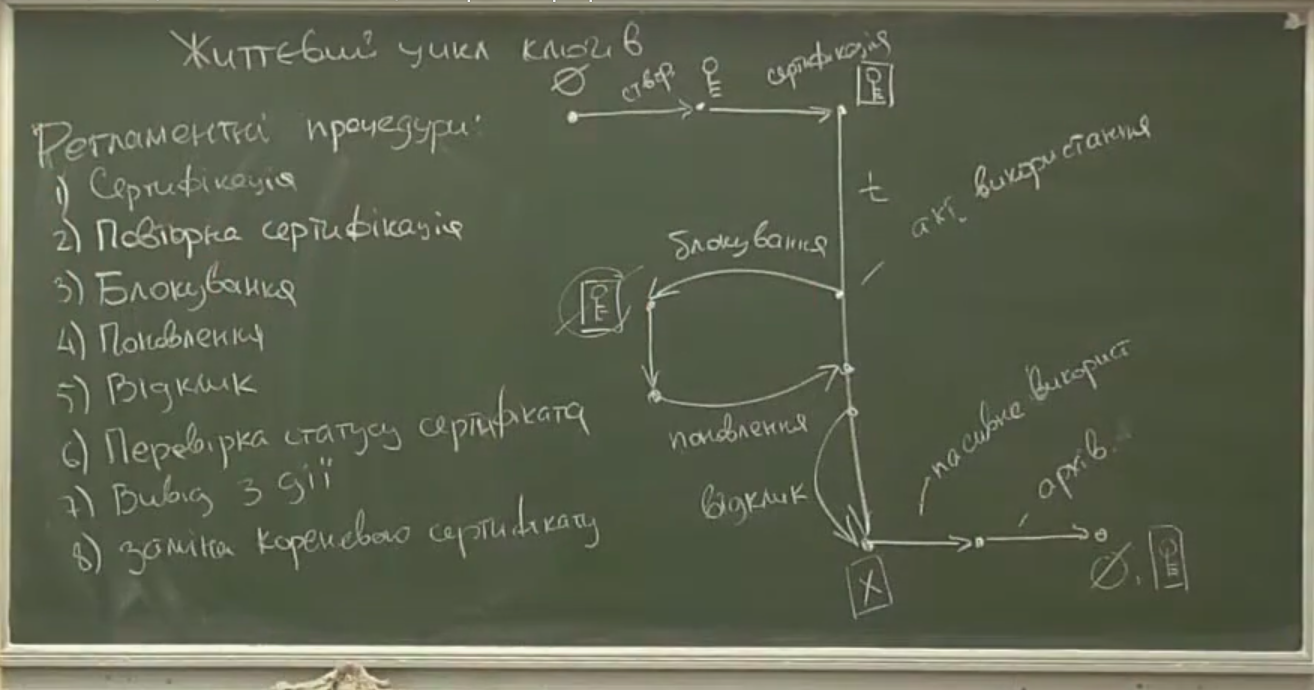
\includegraphics[width=0.45\textwidth]{images/nyakovlev_ivk_rgb.png}
        }
        \subfloat[Оператор Лапласа + Бінаризація Отсу]{
            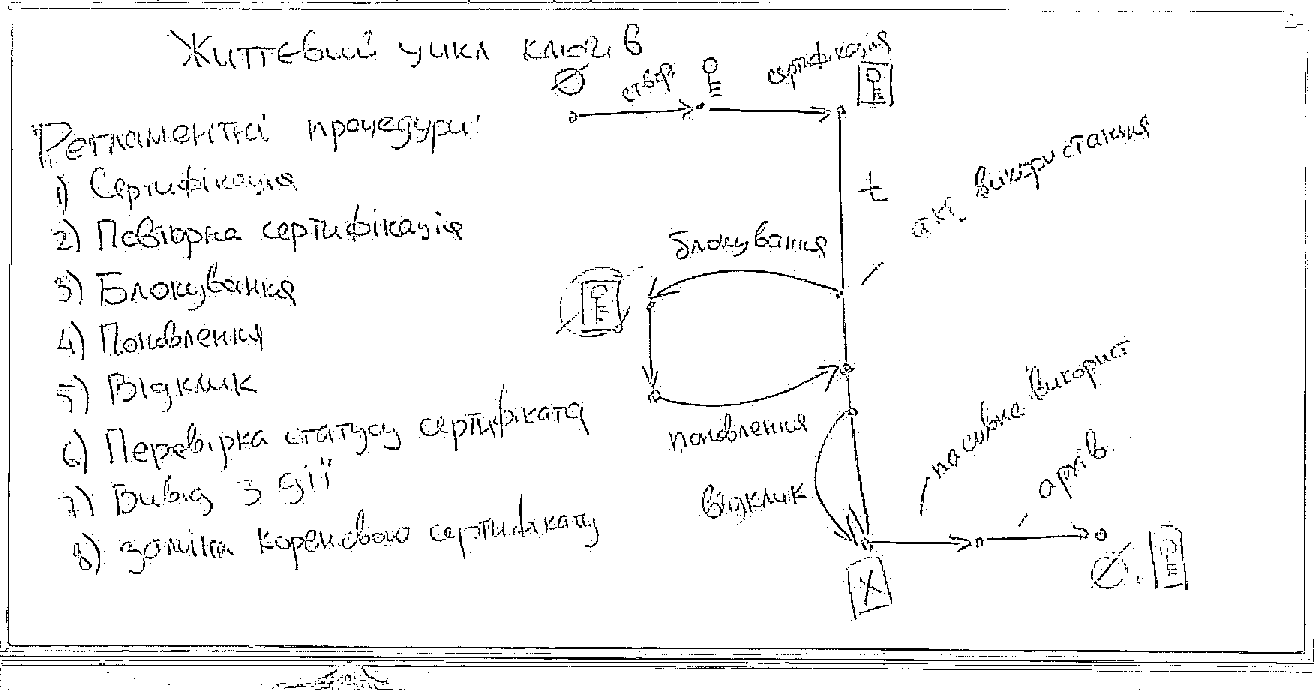
\includegraphics[width=0.45\textwidth]{images/nyakovlev_ivk_bin.png}
        }
        \caption{Джерело ~---~ \url{https://youtu.be/vlKvBax6nHY}}
    \end{figure}
\end{frame}

\begin{frame}
    \frametitle{Обробка слайдів}
    \begin{figure}[H]
        \centering
        \subfloat[До швидкої медіани]{
            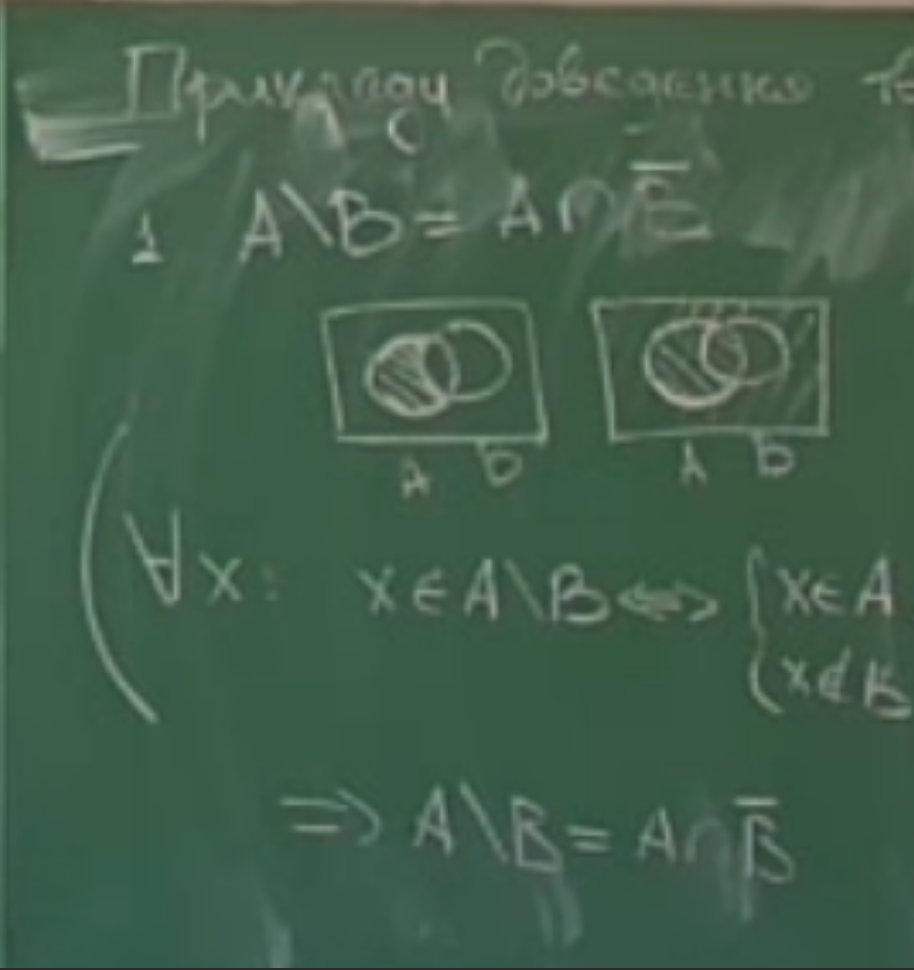
\includegraphics[width=0.25\textwidth]{images/frame_before_median}
        }
        \subfloat[Після швидкої медіани]{
            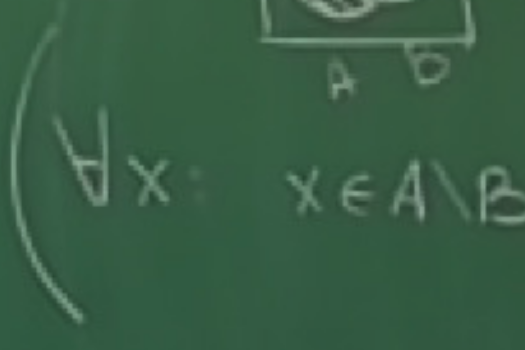
\includegraphics[width=0.25\textwidth]{images/frame_after_median}
        }
    \end{figure}
\end{frame}

\section{Висновки}
\begin{frame}
  \frametitle{Висновки}
  \begin{itemize}
    \item В результаті виконання роботи вдалося розробити алгоритм створення панорамних слайдів без викладача.
    \item Виявлено, що алгоритм Бойкова-Колмогорова досить добре справляється у задачі видалення рухомих об'єктів.
          Результати роботи згорткових нейромереж сімейства YOLO, MobileNet, SSD та
          R-CNN свідчать про високу якість детекції людини та можливість
          їх використання на смартфонах. За експериментальними результатами YOLOv5n є найбільш оптимальним
          методом прибирання викладача.
    \item Було реалізовано програмне забезпечення,
          що приймає на вхід відео з параметрами від користувача та
          будує панорамні оброблені слайди.
    \item Якість результатів слайдів свідчить про необхідність проведення подальшої роботи та
          ще покращення алгоритму й інформаційної технології. Наприклад детекція дошки прискорить
          роботу системи, оскільки розмір панорами зменшиться і потрібно буде менше часу для її обробки.
  \end{itemize}








\end{frame}

\end{document}
